
\begin{figure}
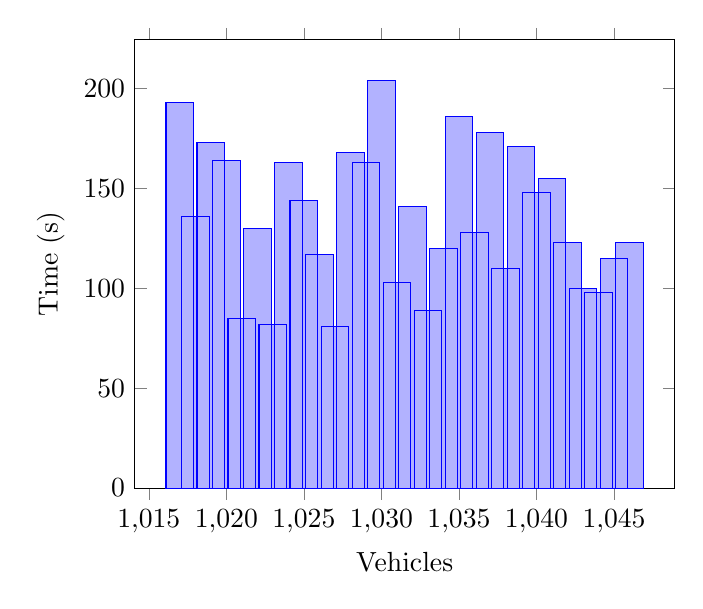
\begin{tikzpicture}
\begin{axis}[
legend style={anchor=west},
xlabel=Vehicles,
ylabel=Time (s),
ymin=0,
ybar,
]
\addplot coordinates {
(1017, 193)
(1025, 144)
(1028, 168)
(1043, 100)
(1032, 141)
(1042, 123)
(1041, 155)
(1040, 148)
(1046, 123)
(1045, 115)
(1044, 98)
(1037, 178)
(1018, 136)
(1019, 173)
(1023, 82)
(1022, 130)
(1029, 163)
(1038, 110)
(1033, 89)
(1031, 103)
(1035, 186)
(1039, 171)
(1036, 128)
(1030, 204)
(1024, 163)
(1027, 81)
(1026, 117)
(1021, 85)
(1020, 164)
(1034, 120)
};

\end{axis}
\end{tikzpicture}
\label{tik:time:100:97}
\caption{100 percent diving with GSC on route $97$}
\end{figure}
